
\documentclass[
  unknownkeysallowed %  ignore keyval errors (produced by Lato font)
]{beamer}

\usepackage[T1]{fontenc}
\usepackage[utf8]{inputenc}
\usepackage[spanish]{babel}

\usepackage{pgf,pgfpages}
\usepackage{tikz}
\usetikzlibrary{arrows,shapes,backgrounds,calc}

\usepackage{graphicx}
\usepackage{colortbl}

%% Beamer style.....
\mode<presentation>
{
  \usetheme{PHD}
  \setbeamercovered{transparent}
  \setbeamertemplate{items}[square]
}

%\usefonttheme[onlymath]{serif}

\beamertemplatenavigationsymbolsempty

\defbeamertemplate{enumerate item}{mycircle}
{
  %\usebeamerfont*{item projected}%
  \usebeamercolor[bg]{item projected}%
  \begin{pgfpicture}{0ex}{0ex}{1.5ex}{0ex}
    \pgfcircle[fill]{\pgfpoint{-0.1pt}{.65ex}}{1.1ex}
    \pgfbox[center,base]{\color{PHDyellow}{\insertenumlabel}}
  \end{pgfpicture}%
}
[action]
{\setbeamerfont{item projected}{size=\scriptsize}}
\setbeamertemplate{enumerate item}[mycircle]

%..............beamer style

\newcommand{\strip}[1]{%
  \begin{flushright}
    \color{PHDgrayC}
    \scriptsize{#1}
\end{flushright}}

\title[C\'adiz Num\'erica 2013]
{Las Matemáticas y el <<Mundo Real>>}
\author[J. R. Rguez. Galv\'an]{%
  { J. Rafael Rodr\'{\i}guez Galv\'an}
  \\[1.5em]
  {\small \em Colegio Argantonio}
  \\[0.2em]
  {\scriptsize Cádiz, \today}
}
\date{}

% XeLaTeX font choosing
% \usepackage{fontspec}%{xltxtra} %fontspec}
% \setsansfont{Fontin Sans}
% \setsansfont{Lato}

% PDFLaTeX font choosing
\usepackage[math, default, scale=1.0]{lato}
% \usepackage[math, default, scale=0.95]{vollkorn}

% Different math fonts, see http://tug.org/pracjourn/2006-1/hartke/hartke.pdf
%\usepackage{eulervm}
%\usepackage{ccfonts, eulervm}
%\usepackage[math]{kurier}
%\usepackage[math]{anttor}
%\usepackage{pxfonts}
%\usepackage{mathpazo}
%\usepackage{mathpple}
%\usepackage[varg]{txfonts}
%\usepackage{arev}
%\usepackage{fourier}

\usepackage{tabularx}
\usepackage{array, multirow, booktabs, rotating} % booktabs: toprule, midrule...



%\newtheorem{remark}{Remark}
%\newtheorem{theorem}{Theorem}

\newcommand\gris{\color{PHDgray}}
\newcommand\amarillo{\color{PHDyellow}}

\setcounter{tocdepth}{1}


%======================================================================
\begin{document}
%======================================================================

%
% Portada ............................................................
%
\setbeamertemplate{background}
 {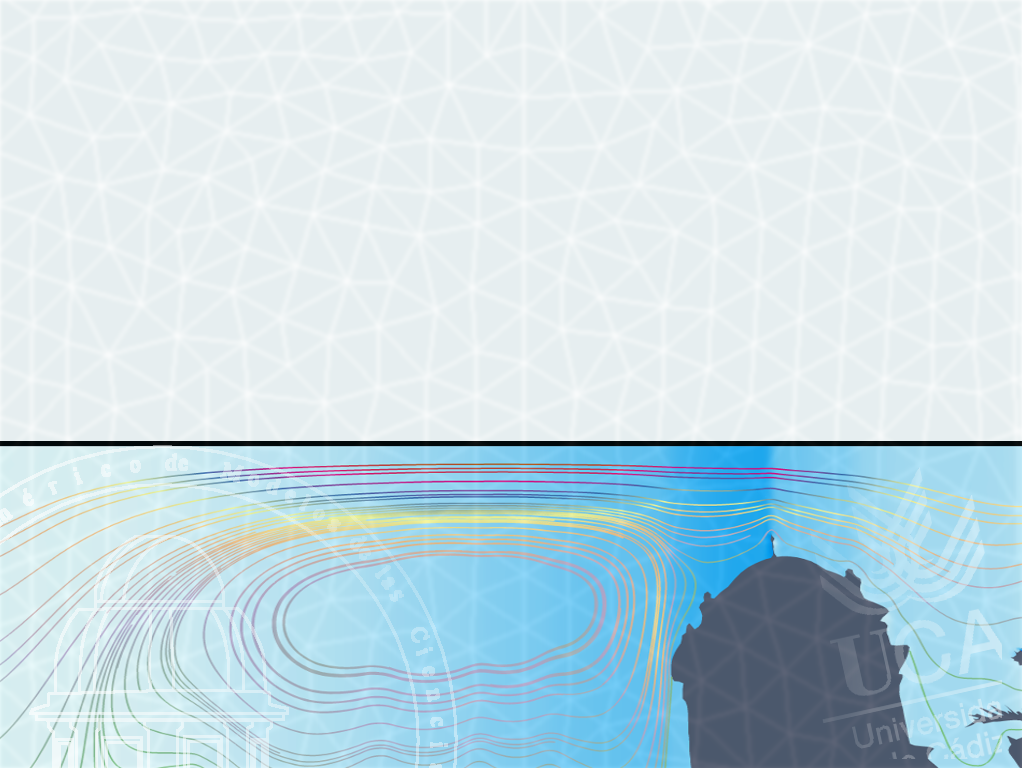
\includegraphics[width=\paperwidth,height=\paperheight]{frontpage_bg}}
\setbeamertemplate{footline}[default]

% Write custom titlepage ------->>>
\begin{frame}
  \titlepage
  \vspace{2.5cm}
\end{frame}

%
% Contenidos ............................................................
%

% Set the background for the rest of the slides.
\setbeamertemplate{background}
 {
\includegraphics[width=\paperwidth,height=\paperheight]{slide_bg}}

\begin{frame}{Plan}
  \tableofcontents
\end{frame}

\section{Introducción}

\begin{frame}{El mundo de las ideas y mundo real}
  \begin{minipage}{0.45\linewidth}
    % \begin{tikzpicture}
    %   \draw
    %   (3,-1) coordinate (a) node[right] {a}
    %   -- (0,0) coordinate (b) node[left] {b}
    %   -- (2,2) coordinate (c) node[above right] {c}
    %   pic["$\alpha$", draw=orange, <->, angle eccentricity=1.2, angle radius=1cm]
    %   {angle=a--b--c};
    % \end{tikzpicture}
    \begin{center}
      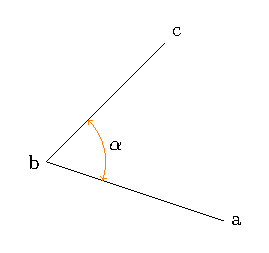
\includegraphics[width=0.65\linewidth,height=0.55\linewidth]{img/angles-quotes}
    \end{center}
    \begin{align*}
      (a-b)(a+b)=a^2-b^2
      \\[3em]
    \int_a^b f(x) \; dx = F(b)-F(a)
    \end{align*}
  \end{minipage}
  \qquad
  \begin{minipage}{0.45\linewidth}
    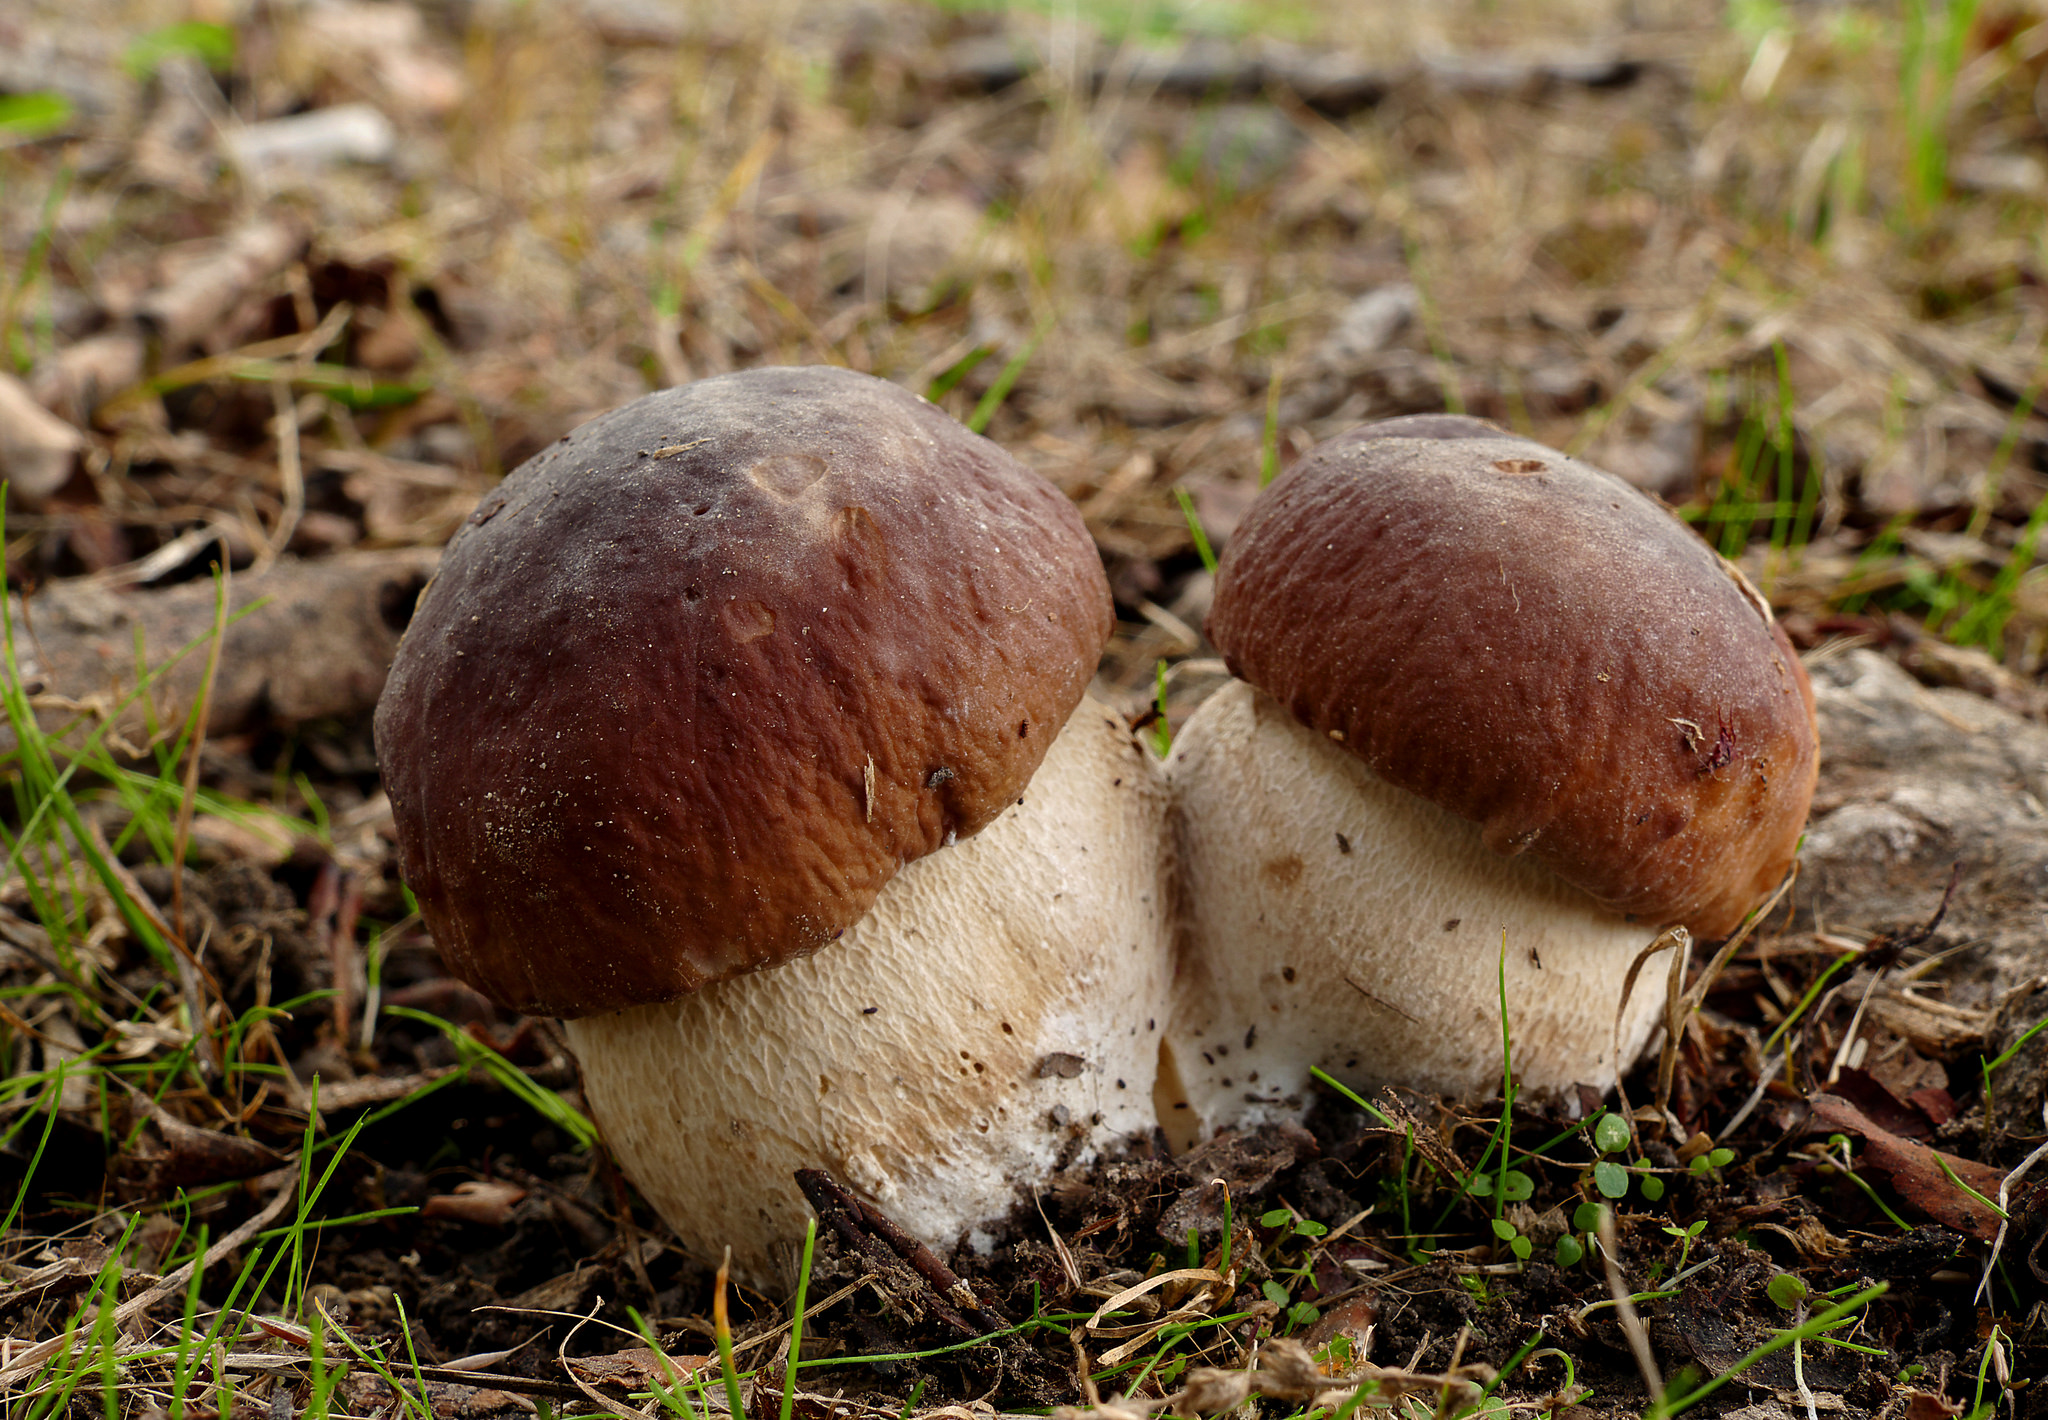
\includegraphics[width=0.8\linewidth]{img/setas}
    \\[-1.5em]
    \hspace*{2em}%
    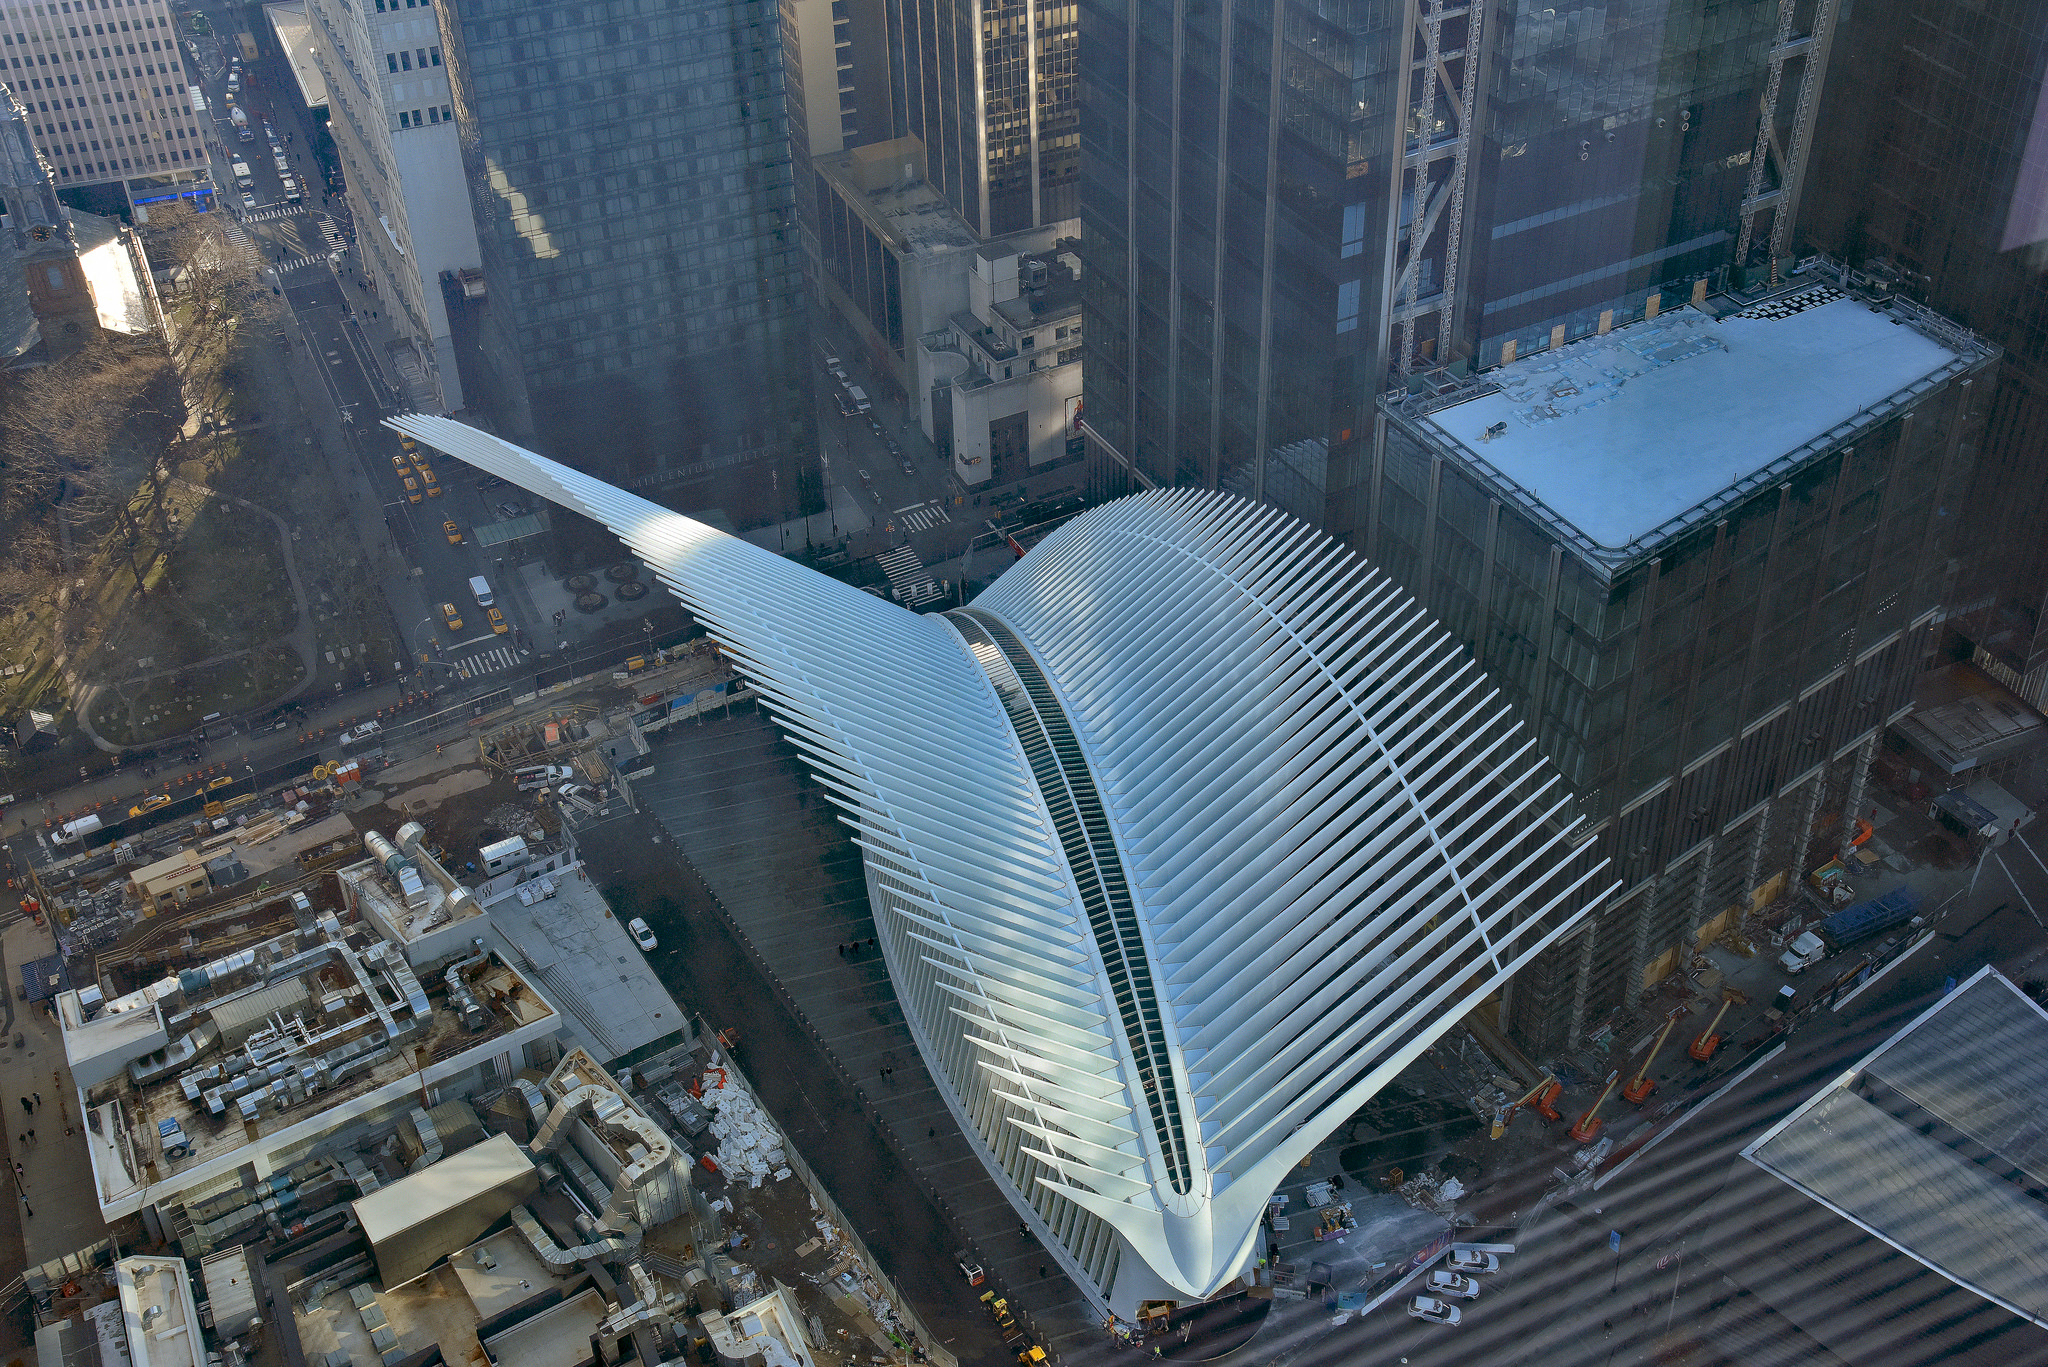
\includegraphics[width=0.8\linewidth]{img/world-trade-center}
    \\[-1em]
    \hspace*{3.5em}%
    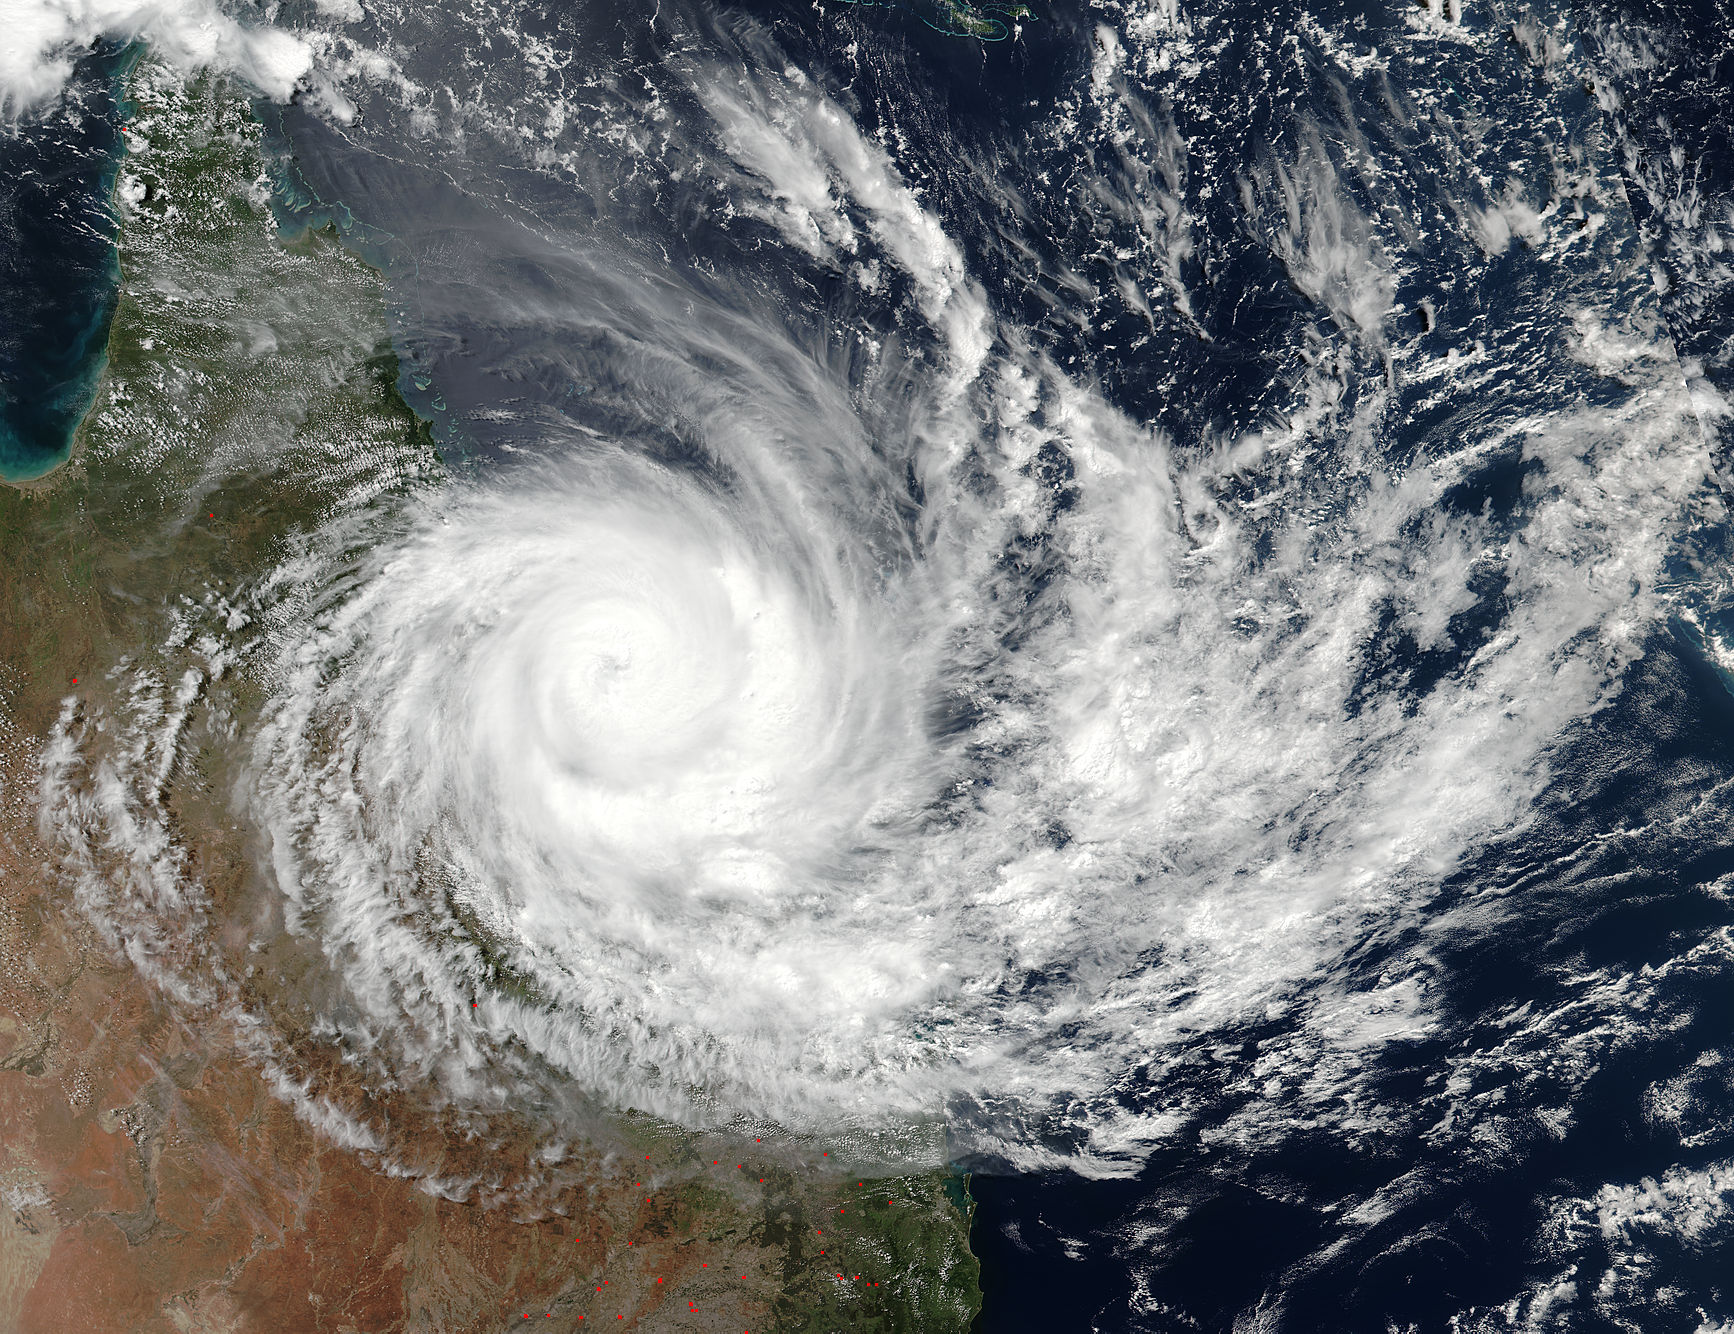
\includegraphics[width=0.8\linewidth]{img/ciclon}
  \end{minipage}
  \begin{minipage}{0.45\linewidth}
  \end{minipage}
\end{frame}

\begin{frame}{Modelos Matemáticos}

\end{frame}

\begin{frame}{Imágenes utilizadas}
  \scriptsize
  \begin{enumerate}
  \item Tropical Cyclone Debbie Make Landfall in Queensland. NASA, licencia CC-by.
  \item King Boletes (Boletus edulis). Bernard Sprag, dominio público.
  \item One World Trade Center\_2016. Harvey Barrison, licencia CC by-sa.
  \end{enumerate}
\end{frame}

\end{document}

%%% Local Variables:
%%% coding: utf-8
%%% TeX-master: t
%%% mode: latex
%%% ispell-local-dictionary: "spanish"
%%% End:
